%TCIDATA{Version=5.50.0.2960}
%TCIDATA{LaTeXparent=0,0,sw-edit.tex}
                      

\subsection{Questionnaire for users of the Google Opinion Rewards mobile app}

Users of the app choose to participate (Figure~\ref{fig:app:intro}). They then get the same questions, but are not offered an explicit option to exit (Figures~\ref{fig:app:q1}-\ref{fig:app:q3}). They can, of course, leave the app at any time. At the end of the survey, the amount of credit earned is shown (Figure~\ref{fig:app:exit}). It is unknown if any credit is earned if users break off the survey. The amount is not determined by the researcher, and cannot be modified. 

\begin{figure}
	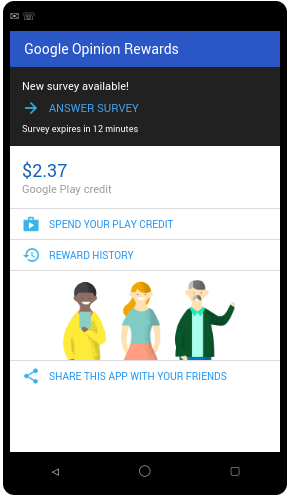
\includegraphics{Selection_360.png}
	\caption{\label{fig:app:intro}Invitation to participate for app users}
\end{figure}
\begin{figure}
	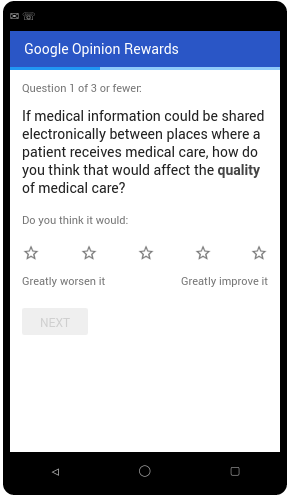
\includegraphics{Selection_361.png}
	\caption{\label{fig:app:q1}Question 1: Quality of Medical Care (app)}
\end{figure}
\begin{figure}
	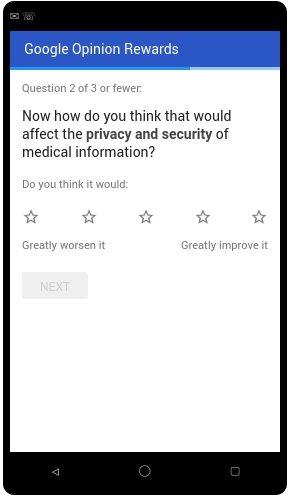
\includegraphics{Selection_362.png}
	\caption{\label{fig:app:q2}Question 2: Privacy (app)}
\end{figure}
\begin{figure}
	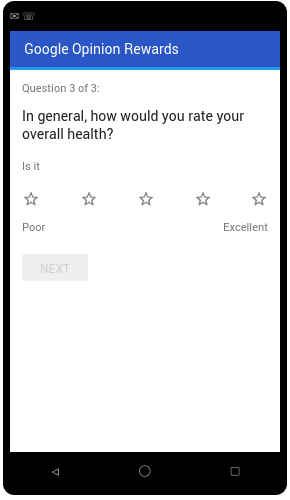
\includegraphics{Selection_363.png}
	\caption{\label{fig:app:q3}Question 3: Health overall (app)}
\end{figure}

\begin{figure}
	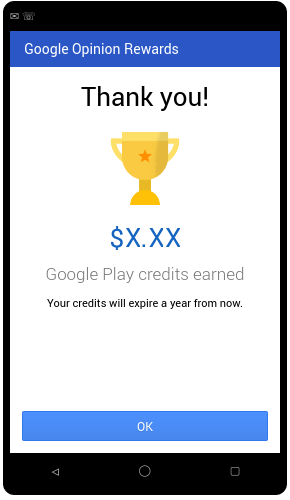
\includegraphics{Selection_364.png}
	\caption{\label{fig:app:exit}Exit screen for app users}
\end{figure}

\FloatBarrier
\subsection{Google Privacy Policy}
\label{sec:gcs_privacy}
The following copy of Google's Privacy Policy was downloaded on 2017-04-14.

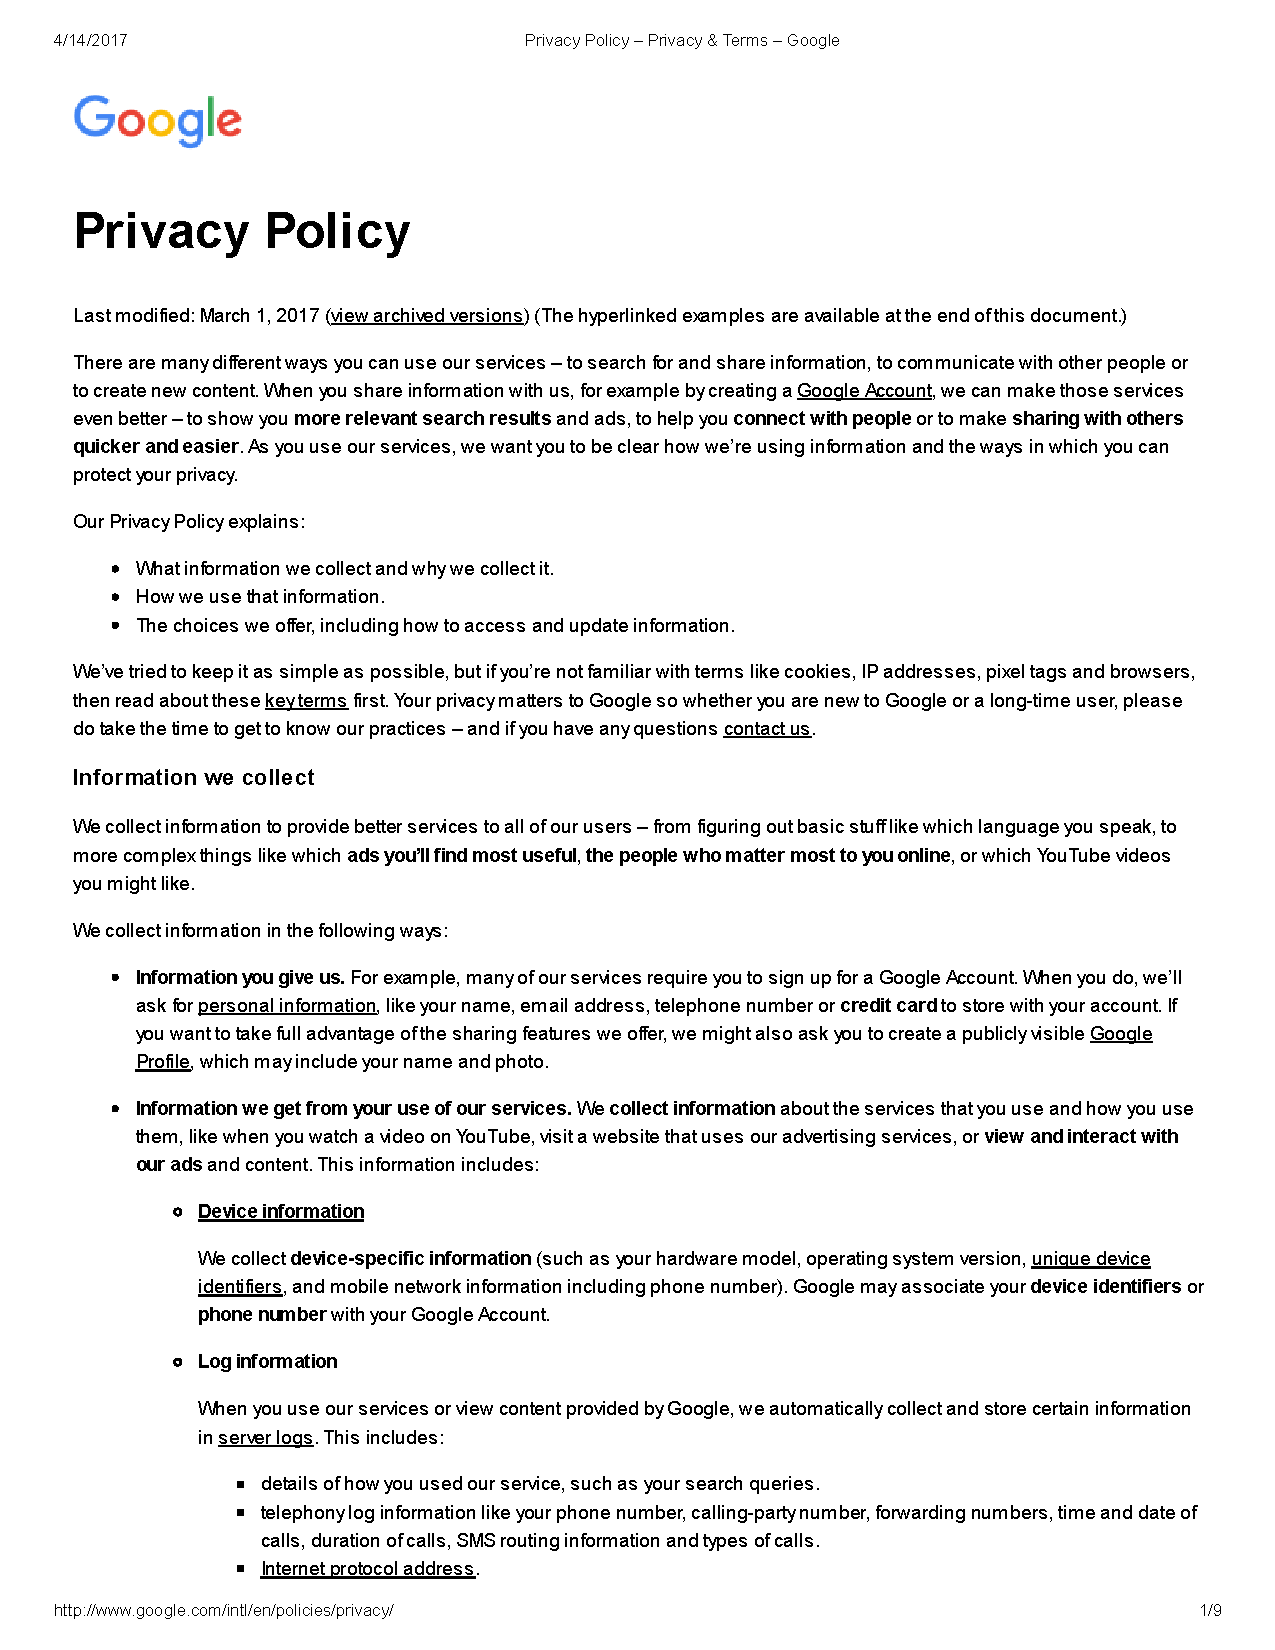
\includepdf[pages=-]{Privacy_Policy_Google_20170414.pdf}
